\documentclass[a4paper]{article}
\usepackage{graphicx}
\usepackage{float}
\author{Hein van Beers, Jeroen van Hoof}
\title{Automated Reasoning\\
	 \large Practical assignment, Part I}
\begin{document}
	\maketitle
	
	\section*{Problem 1: Delivery for magic factory}
	Satisfying all constraints, find the maximum number of pallets of prittles that can be delivered, and show how for that number all pallets may be divided over the six trucks.

	
	\section*{Solution:}
	We generalize this problem to $n$ trucks. For each pallet place in a truck we introduce five variables, one for each type of building block. We have eight pallet places per truck, so we introduce $8*5*n = 40*n$ variables $p_{ijk}$ for $i = 1,\ldots,n$, $j = 1,\ldots,8$ and $k = 1,\ldots,5$ where for every $i,j,k$ the value of $p_{ijk}$ will be true if and only if a pallet of building block type $k$ will be put on pallet position $j$ in truck $i$.
	
	As the weight of each of the $n$ trucks may not exceed the capacity of 7800 kg, we express this by the formula
\[ \bigwedge_{i=1}^n (\sum_{k=1}^5 (\sum_{j=1}^8 (p_{ijk}*w_k)) \leq 7800).\]
Where $w_k$ is the weight of a pallet of type $k$. In the table below you can see the values of the different types of pallets.

\begin{table}[H]
\centering
\caption{Weights of the different types of pallets}
\label{my-label}
\begin{tabular}{c|c|c}
\textbf{Pallet type} & \textbf{Corresponding k} & \textbf{Weight (kg)} \\ \hline
Nuzzles              & 1                        & 700                  \\ \hline
Prittles             & 2                        & 800                  \\ \hline
Skipples             & 3                        & 1000                 \\ \hline
Crottles             & 4                        & 1500                 \\ \hline
Dupples              & 5                        & 100                 
\end{tabular}
\end{table}

	As prittles and crottles are not allowed to be put in the same truck, that is, for every two distinct positions $j,m$ in truck $i$ it is not allowed that both $p_{ij2}$ and $p_{im4}$ are true. This is expressed by the formula
\[ \bigwedge_{i=1}^n (\neg (\bigvee_{j=1}^8 p_{ij2}) \vee \neg (\bigvee_{m=1}^8 p_{im4})).\]

Next we assume that the first two trucks are cooled, so pallets of skipples cannot be placed in trucks 3 upto and including $n$. We express this by the formula
\[ \bigwedge_{i=3}^n \bigwedge_{j=1}^8 \neg p_{ij3}.\]

No two pallets of the type dupples may be placed in the same truck, that is, for every two distinct positions $j,m$ in truck $i$ it is not allowed that both $p_{ij5}$ and $p_{im5}$ are true. This is expressed by the formula
\[ \bigwedge_{i=1}^n \bigwedge_{j,m:1 \leq j < m \leq 8} \neg p_{ij5} \vee \neg p_{im5}.\]

Similarly, we also need the requirement that at most one variable is set to true per pallet position in a truck. So for every two distinct pallet types $k,m$ on position $j$ in truck $i$ it is not allowed that both $p_{ijk}$ and $p_{ijm}$ are true. This is expressed by the formula
\[ \bigwedge_{i=1}^n \bigwedge_{j=1}^8 \bigwedge_{k,m:1 \leq k < m \leq 5} \neg p_{ijk} \vee \neg p_{ijm}.\]

Finally, we consider the requirements of the demands.

The total formula now consists of the conjunction of all these ingredients, that is,


This formula is easily expressed in SMT syntax, for instance, for
$n=6$ one can generate

{\footnotesize

{\tt (benchmark test.smt}

{\tt :extrapreds (}

{\tt (p11) (p12) (p13) (p14) (p15) (p16) (p17) (p18) }

{\tt (p21) (p22) (p23) (p24) (p25) (p26) (p27) (p28) }

{\tt (p31) (p32) (p33) (p34) (p35) (p36) (p37) (p38) }

{\tt (p41) (p42) (p43) (p44) (p45) (p46) (p47) (p48) }

{\tt (p51) (p52) (p53) (p54) (p55) (p56) (p57) (p58) }

{\tt (p61) (p62) (p63) (p64) (p65) (p66) (p67) (p68) }

{\tt (p71) (p72) (p73) (p74) (p75) (p76) (p77) (p78) }

{\tt (p81) (p82) (p83) (p84) (p85) (p86) (p87) (p88) }

{\tt )}

{\tt :formula}

{\tt   (and}

{\tt (or (p11) (p12) (p13) (p14) (p15) (p16) (p17) (p18) )}

{\tt (or (p21) (p22) (p23) (p24) (p25) (p26) (p27) (p28) )}

$\cdots \cdots$

{\tt (or (not p11) (not p12)) }

{\tt (or (not p11) (not p13)) }

$\cdots \cdots$

{\tt )) }
}

Applying {\tt yices -e -smt test.smt} yields the following result
within a fraction of a second:

{\footnotesize

{\tt sat }

{\tt (= p11 false)}

{\tt (= p12 false)}

{\tt (= p13 false)}

{\tt (= p14 true)}

{\tt (= p15 false)}

{\tt (= p16 false)}

{\tt (= p17 false)}

{\tt (= p18 false)}

{\tt (= p21 false)}

{\tt (= p22 true)}

{\tt (= p23 false)}

$\cdots \cdots$ }.

The values that are are true are $p_{14}, p_{22}, p_{37}, p_{43},
p_{56}, p_{68}, p_{75}, p_{81}$. Expressed in a picture this
yields

\begin{figure}[H]
			\centering
				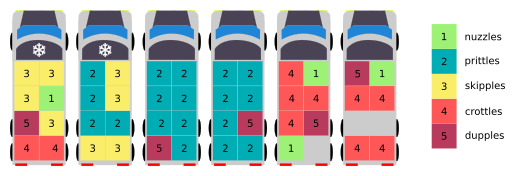
\includegraphics[scale=1]{trucks.png}
			\caption{Placement of pallets on truck. The first two trucks have facility for cooling skipples.}
		\end{figure}

We check that indeed there are eight queens for which no two are
on the same row, column or diagonal.

\vspace{3mm}

{\bf Remark:} 

Our formula contains some redundancy: the requirement that every
row contains exactly one queen implies that there are exactly $n$
queens in total. By expressing that every column contains at least
one queen, from this property one concludes that also every column
contains at most one queen. We chose for this redundancy for
keeping the symmetry in the solution, and also following the
general strategy that introducing redundancy is often good for
efficiency.

\vspace{3mm}

{\bf Generalization:} 

As we generalized our approach for $n$ rather than 8, it is
interesting to see what happens for other values of $n$. For $n
> 10$ we have to take care of the notation: if we keep the
notation then it is not clear whether {\tt p111} represents 
$p_{1,11}$ or $p_{11,1}$. This is solved by putting an extra 
symbol between the two numbers. 

For $n=3$ the resulting formula is unsatisfiable, showing that
there is no solution. For $n = 4,5,6,\ldots$ the formula is
satisfiable, by which is a solution of the problem is found.
Efficiency is not a problem: for $n = 60$ there are 3600
variables and the formula consists of over 350,000 clauses, but 
still {\tt yices} succeeds in finding a solution within a few
seconds.
	\section{Problem 2}
	\begin{figure}[H]
		\centering
			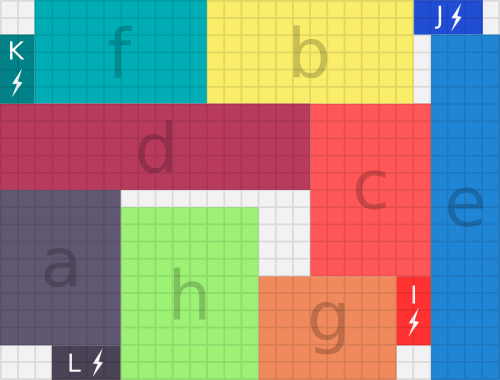
\includegraphics[scale=0.5]{power-grid-2.png}
		\caption{Placement of components on chip.}
	\end{figure}
	\section{Problem 3}
	\begin{figure}[H]
		\centering
			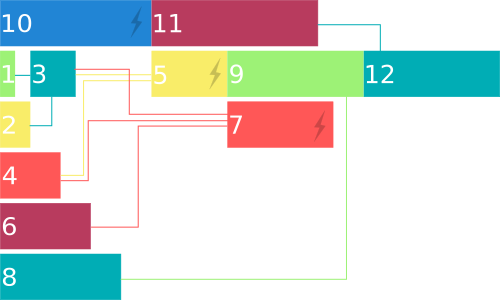
\includegraphics[scale=0.7]{timeline.png}
		\caption{Time-line of process execution. Connected processes depend on each other, special processes are marked with a sign.}
	\end{figure}

\end{document}